\subsubsection{Hyperlink-Tarpit}
Die erste der drei implementierten Tarpitformen ist die klassische HTTP-Tarpit, wie sie auch unter Punkt \ref{subsub:http-tarpit} beschrieben ist. Hierbei werden fortlaufend neue Hyperlinks generiert, welche allesamt \glqq ins Leere\grqq,\space sprich auf keine weitere Webseite, zeigen. Dies würde bei einem herkömmlichen Webserver einen \emph{404 Not Found} HTTP-Statuscode hervorrufen, welcher dem Aufrufer mitteilt, dass die angeforderte Ressource, sprich die Webseite, auf dem Webserver nicht existiert. Ein vermehrtes auftreten von solchen 404-Codes würde einen Webcrawler alarmieren und er würde den Crawl-Vorgang abbrechen, da er der Meinung ist, auf diesem Webserver gäbe es nichts zu holen. Um dies zu verhindern muss dem Webserver mitgeteilt werden, dass wir bei einem 404-Code gerne eine eigene Seite anzeigen möchten. Dies kann bei Apache durch den Befehl
\begin{lstlisting}
ErrorDocument 404 [ADRESSE]
\end{lstlisting} 
erledigt werden. Diesen Befehl kann man dann sowohl in der Datei \emph{.htaccess} festlegen als auch in der Datei \emph{000-default.conf}, welche sich in Linux-Systemen unter dem Pfad \emph{/etc/apache2/sites-available/000-default.conf} befindet. Bei der Änderung der .conf-Datei ist jedoch Vorsicht geboten und es empfiehlt sich vorher ein Backup zu machen. Für den weiteren Verlauf dieses Projektes sollen alle 404-Codes auf die Datei \emph{reply.php} umgeleitet werden:
\begin{lstlisting}
ErrorDocument 404 /reply.php
\end{lstlisting}
Das PHP-Skript, welches in der Datei \emph{reply.php} enhalten ist, generiert dann eine Webseite mit zufälligem Text, welcher wiederum zufällige Hyperlinks enthält. Als aller erstes muss jedoch der 404-Statuscode vom Webserver unterbunden werden. Denn der zuvor aufgeführte Code leitet nur die Anfrage an die Datei reply.php weiter, behält jedoch den Statuscode, in diesem Fall 404, bei. Um den Statuscode zu ändern muss das PHP-Skript den Statuscode überschreiben und dem Aufrufer den HTTP-Statuscode \emph{200 OK} senden. Dies passiert in den folgenden Zeilen, welche am Beginn des PHP-Skriptes stehen und den HTTP-Header manipulieren:
\lstinputlisting[language=PHP, firstline=1, lastline=10]{sourcefiles/reply.php}
Da sich der Inhalt der durch das Skript generierten Webseite bei jedem Aufruf ändert, darf es nicht im Cache gespeichert werden.\footnote{Moderne Browser speichern, man spricht hier von cachen, Dateien für einen gewissen Zeitraum, damit sie bei einer erneuten Anfrage nicht erneut vom Webserver heruntergeladen werden müssen und somit Zeit und Traffic gespart wird.} Das Cachen der Webseite ist in diesem Fall schlecht, da es einen Webcrawler am Generieren von neuem Inhalt hindern könnte. Dies wird ebenfalls durch den zuvor aufgeführten Codeteil gewährleistet, da er sowohl das Änderungs-, als auch das Verfallsdatum für die Speicherung im Cache auf das aktuelle Datum setzt. Diese Zeitangaben muss in der Greenwich Mean Time\footnote{Die Greenwich Mean Time (GMT) ist die Zeitzone, welche in Greenwich/London gilt.} angegeben werden.\cite{http-header-time} Des Weiteren schreibt er ein \emph{no-store}, \emph{no-cache} und \emph{must-revalidate} vor, welche allesamt dem Aufrufer das Cachen der Webseite untersagt.\\
Das Skript generiert anschließend eine Webseite, welche aus drei unterschiedlich langen Spalten besteht. Die Spalten werden anschließend mit Buchstaben, Wörtern und Zeichen befüllt. Die Verteilung der Buchstaben entspricht dabei ungefähr den realen Werten der englischen Sprache. Hierfür wurde ein Array erstellt, in welchem die Buchstabe anhand der Verteilung der Buchstaben in der englischen Sprache aufgelistet sind.\footnote{Eine Tabelle der Verteilung der Buchstaben kann unter \url{http://kryptografie.de/kryptografie/kryptoanalyse/haeufigkeitsverteilung.htm} eingesehen werden.}
 Dies bedeutet, wenn ein Buchstabe beispielsweise eine sechs-prozentige Verteilung in der englischen Sprache aufweist, so belegt er auch sechs Prozent der verfügbaren Arrayplätze. Um die generierte Webseite noch realistischer wirken zu lassen und somit keinen Anschein einer Tarpit zu erwecken, wurden folgende Konzepte umgesetzt:
\begin{description}
	\item[Generieren von \grqq echten\grqq\space Wörter] Es werden neben den zufällig generierten Buchstaben auch noch vordefinierte englische Wörter\footnote{Beispiele für vordefinierte englische Wörter wären \emph{the}, \emph{be}, \emph{and} usw..}, Satzzeichen und Leerzeichen mit unterschiedlicher Wahrscheinlichkeit zum Text hinzugefügt. Durch das Einfügen von Leerzeichen entstehen weitere \grqq wörterähnliche\grqq\space Strukturen.
	\item[Variieren der Spaltenlänge] Die generierte Webseite besitzt drei Spalten, welche jeweils eine unterschiedliche Länge aufweisen. Eine Längeneinheit ist hierbei ein Zeichen oder ein vordefiniertes Wort. Die Länge der Spalten bewegt sich hierbei zwischen 3.000 und 4.000 Zeichen bzw. vordefinierte Wörter.
	\item[Generieren von Hyperlinks] Auf einer Webseite befinden sich durchschnittlich 6,4 Hyperlinks, welche auf einen anderen Bereich der Seite, eine komplett andere Webseite oder auf eine andere Domain zeigen.\cite{tarpitting-http-linux-mag} Je mehr Hyperlinks auf einer Webseite sind, umso effizienter kann man einen Webcrawler für eine Zeit lang \glqq beschäftigen\grqq . Damit die generierte Webseite jedoch trotzdem eine realistische Anzahl an Hyperlinks aufweist, generiert das PHP-Skript mit einer Wahrscheinlichkeit von einem Prozent eine Hyperlink auf einem zufällig generierten Ziel mit einer Länge zwischen 5 und 25 Zeichen. Dies ergibt bei einer Spaltenlänge von 3.000 bis 4.000 Zeichen eine durchschnittliche Hyperlink-Anzahl von 90 bis 120. Um die Struktur der Hyperlinks zu variieren zeigen sie jeweils mit einer Wahrscheinlichkeit von je 25\% auf eine Datei mit der Endung .htm oder .php und mit einer Wahrscheinlichkeit von 50\% auf eine .html-Datei. Die Verteilung dieser Wahrscheinlichkeiten ist nochmals in Abbildung \ref{fig:wahrbaum} auf Seite \pageref{fig:wahrbaum} aufgezeigt.
\end{description}
Somit generiert ein Webcrawler bei jedem Aufruf des Skriptes um die 100 neue Hyperlinks. Ruft er nun $n$-mal dieses Skript auf, so generiert er $100^n$ virtuelle, nicht existente, Dateien. Dies ist eine exponentielle Funktion, welche enorm schnell wächst. Bei sechs-maligem Aufrufen der Seite, was für einen Webcrawler de facto kein Aufwand ist, hat er somit bereits $100^6 = 1.000.000.000.000$ (Eine Billion) Hyperlinks gezeugt, welche in seiner Queue gespeichert sind. Wenn ein Webcrawler theoretisch ein Zehntel einer Sekunde für das Abarbeiten einer Webseite brauchen würde, wäre er hiermit schon über 31.000 Jahre beschäftigt.\\
Ein Webcrawler ist somit schnell gefangen. Sollte ein Webcrawler die Falle bemerken, so wurde zumindest seine Queue unbrauchbar gemacht. Durch ein leeren dieser Queue würde der Webcrawler zwar wieder diese sinnlosen Hyperlinks los werden, jedoch würde er auch alle anderen darin gespeicherten Hyperlinks verlieren.\\
Anzumerken ist jedoch, dass die oben angegebenen Zahlen nur einem theoretischen Wert entsprechen und das Skript in der Praxis mit einer Wahrscheinlichkeit von 10\% anstelle der \glqq normalen\grqq\space Hyperlinks eine E-Mail-Adresse geniert, siehe hierfür Punkt \ref{subsub:harverster-tarpit}.\\
\begin{figure}[H]
	\centering
	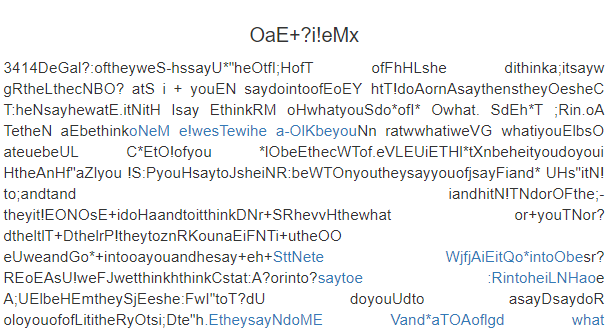
\includegraphics[width=8.45cm]{img/beispiel-hyperlink1.PNG}
	\caption{Beispielausgabe des Skriptes \emph{reply.php}. Zur besseren Übersicht wird nur eine der drei Spalten angezeigt}
	\label{fig:beispiel-hyperlink}
\end{figure}
Das gesamte reply.php-Skript ist in den Anhängen beigefügt und einsehbar.
\label{subsub:hyperlink-tarpit}

